\graphicspath{{bv02_Buchstabieren+Funken/}}

% \clearpage
% \begin{minipage}{0.8\textwidth}
   \chapter{Internationales Buchstabieralphabet (BV02)}
% \end{minipage}
% \begin{minipage}{0.2\textwidth}
%   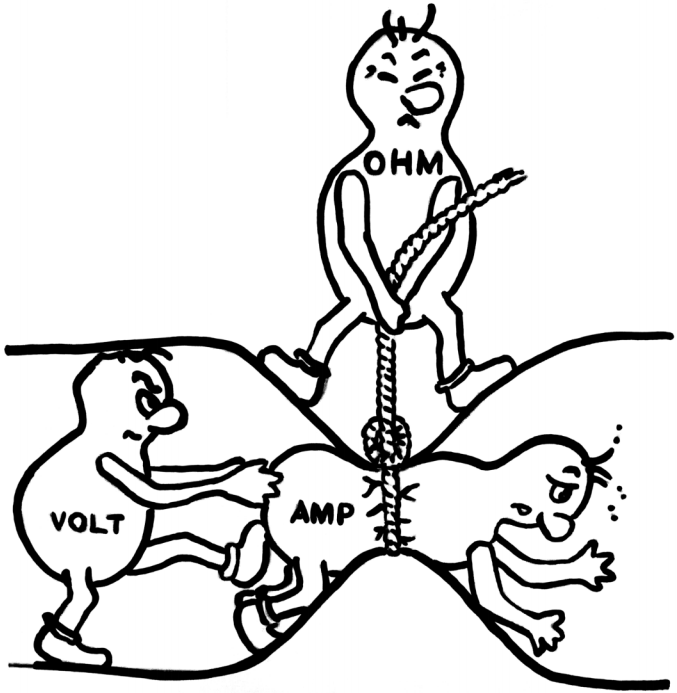
\includegraphics[width=0.9\textwidth]{URI.png}
%   \footnotemark
% \end{minipage}
% \footnotetext{Quelle unbekannt}

%%%%%%%%%%%%%%%%%%%%%%%%%%%%%%%%%%%%%%%%%%%%%%%%%%%%%%%%%%%%%%%%%%%%%%%%
%% Theorie

\section{Lernvorlage Buchstabiertafel (ITU Phonetic Alphabet)}

\begin{minipage}[t]{0.5\textwidth}
  \large
  \textbf{A}lpha\\
  \textbf{B}ravo\\
  \textbf{C}harly\\
  \textbf{D}elta\\
  \textbf{E}cho\\
  \textbf{F}oxtrott\\
  \textbf{G}olf\\
  \textbf{H}otel\\
  \textbf{I}ndia\\
  \textbf{J}uliett\\
  \textbf{K}ilo\\
  \textbf{L}ima\\
  \textbf{M}ike\\
\end{minipage}
\begin{minipage}[t]{0.5\textwidth}
  \large
  \textbf{N}ovember\\
  \textbf{O}scar\\
  \textbf{P}apa\\
  \textbf{Q}uebec\\
  \textbf{R}omeo\\
  \textbf{S}ierra\\
  \textbf{T}ango\\
  \textbf{U}niform\\
  \textbf{V}ictor\\
  \textbf{W}hiskey\\
  \textbf{X}-Ray\\
  \textbf{Y}ankee\\
  \textbf{Z}ulu\\
\end{minipage}

%%%%%%%%%%%%%%%%%%%%%%%%%%%%%%%%%%%%%%%%%%%%%%%%%%%%%%%%%%%%%%%%%%%%%%%%
%% Praxis

\clearpage

\section{Sprung in die kalten Wellen: Das erste FM-QSO} % ... ins kalte Spektrum?

Um gleich von Beginn an in die Praxis reinzuschnuppern geht es bei den ersten
Funkkontakten (QSO) darum im Nahbereich auf UKW und gut verständlicher
FM-Modulation erste Funksprüche abzusetzen. Im Fokus steht hierbei neben dem
Kennenlernen die Betriebstechnik, also der Ablauf eines Funkspruchs,
Funkdisziplin sowie das Üben des internationalen Buchstabieralphabets. Dies
dient auch als erste Vorbereitung für die Funkpraxis auf Kurzwelle in der
Clubstation und des "`CQ TU"'-Contests. Ablauf:

\begin{enumerate}
  \item[15] min Standortsuche und Vorbereitung
  \item[60] min Funken und Rückweg
  \item[15] min Auswertung
\end{enumerate}

\paragraph{Vorbereitungsaufgabe}

\emph{-- keine --}
\loesung{Besondere Vorbereitungen:
  \begin{itemize}
    \setlength\itemsep{0em}
    \item Anlage drucken % FIXME Referenz
    \item Mindestens zwei, aber eher mehr UHF-Funkgeräte (da am weitesten verbreitet)
      pro Ausbildungs-Operator mitbringen. Programmierung der CQ TU QRGs (falls
      notwendig): 430.200 (U0), 430.225 (U1), 430.250 (U2), 430.275 (U3) --
      Ausbilder/innen QRV U0
    \item Hinweis: Gruppengröße max. 5; max. 5 Gruppen auf einem Kanal,
      sonst dauert das ewig
  \end{itemize}
}

\paragraph{Material}

\begin{itemize}
  \item[1x] UHF-Funkgerät
  \item[1x] Funkplan \& Logbook (mit Stift natürlich) % FIXME Referenz
\end{itemize}

\paragraph{Hinweise}

Don't Panic -- es ist kein Contest, also piano und Fokus auf sauberen Betrieb!

% TODO Flowchart oder Anleitung eines QSOs (allg. & dir. Anruf) ergänzen?

\paragraph{Aufgaben}

\begin{enumerate}
  \item \textbf{Vorbereitung:} Sucht euch in der Gruppe einen Standort (QTH) und ein
    Lösungswort mit der Länge der Anzahl der Teilnehmenden aus. Jede/r bekommt einen
    Buchstaben zugewiesen und hat die Aufgabe diesen den anderen Stationen in
    Sprechweise des internationalen Buchstabieralphabets zu übermitteln. Nutzt die
    ersten Minuten bis zum Übungsbeginn euren Namen im Buchstabieralphabet
    aufzuschreiben sowie den grundsätzlichen Ablauf eines QSOs mit eurem Operator zu
    besprechen und "`trocken"' zu proben.
  \item \textbf{Gesprächsablauf:} In jedem Durchgang sind das Rufzeichen
    (Call)\footnote{bei Bedarf Call ergänzen durch \emph{Secondary Station
    Identifier} --1 bis --4 \\ Sprich: ``Dash 1 $\sim$ 4''. Alternative deutsche
    Sprechweise: ``Strich 1 $\sim$ 4''.}, der Buchstabe und die Stelle im Wort
    zu übertragen. Auf Nachfrage gilt es ebenso das QTH (z.B.  Raumnummer) sowie
    den eigenen Vorname zu buchstabieren.  Jedes QSO ist zu loggen.  Eine
    beliebige Station startet mit einem allgemeinen Anruf. Nach jedem Durchgang
    ist die QRG freizugeben und die zuvor nicht rufende Station darf allgemein
    oder direkt anrufen. Alles weitere ergibt sich.
    %Tip: Zieht euch Unterstriche für die Anzahl der Personen der Gegenstelle und
    %füllt es nicht vollständig aus, auch wenn ihr es bereits erraten könnt.
\end{enumerate}

\paragraph{Ziel} Der Funkplan ist -- inlusive der Lösungswörter und Namen --
vollständig auszufüllen.
